\begin{frame}[fragile]{Proposed Method} 
\vspace{-0.6cm}

\begin{center}
\begin{tikzpicture}[scale=0.75, every node/.style={scale=0.75}, node distance = 2cm, auto]
   
  \node [outer sep=0cm] (environment) at (0,0)  {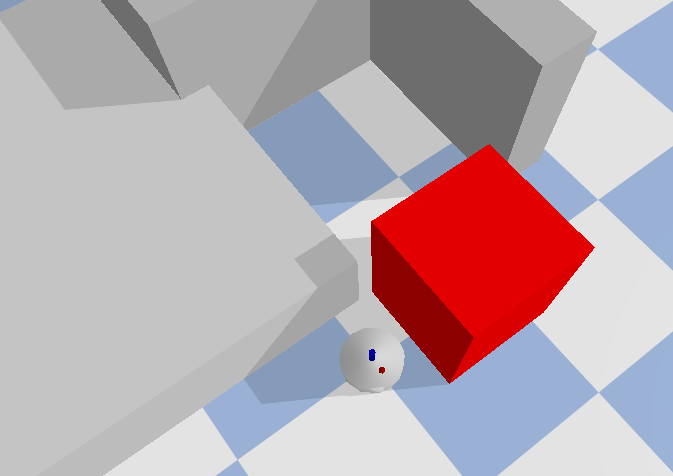
\includegraphics[width=4.6cm]{figures/introduction/robot_no_target}}; 

  \draw [myEvenLighterColor,
  rounded corners=0.3cm, 
  line width=0.3cm]  
  (environment.north west) -- 
  (environment.north east) --
  (environment.south east) --
  (environment.south west) -- cycle  ;

  \node [block,
  above of=environment,
  minimum height=2cm,
  minimum width=5cm,
  node distance=4.1cm,
  outer sep=0cm] (hgraph) {Hypothesis Algorithm};

  \node [block, 
  above of=hgraph, 
  node distance=3.3cm, 
  minimum width=5cm,
  minimum height=2.0cm] (kgraph) {Knowledge Graph};
    
  % Draw edges
  \draw[-stealth] ([yshift=0.155cm, xshift=0.4 cm]environment.north) -- node [xshift=-.05cm, right] {\shortstack[]{sensor\\measurements}}([xshift=0.4 cm]hgraph.south) ;
  \draw[-stealth] ([xshift=-0.4 cm]hgraph.south) -- node [left] {robot input}([yshift=0.155cm, xshift=-0.4 cm]environment.north) ;
  \draw[stealth-] (hgraph.west) -- node [above] {task} ++(-1, 0);


  \draw[-stealth] ([xshift=-0.4cm]kgraph.south) -- node [left] {\shortstack[]{action\\suggestions}}([xshift= -0.4cm]hgraph.north) ;
  \draw[stealth-] ([xshift=0.4cm]kgraph.south) -- node [right] {\shortstack[]{action\\feedback}}([xshift= 0.4cm]hgraph.north) ;
\end{tikzpicture}
\end{center}

\end{frame}


\begin{frame}[fragile]{Proposed Method} 
$G^\mathit{hypothesis} = \left\langle \gls{nodesH}, \gls{edgesH} \right\rangle $
\vspace{0.5cm}
\begin{center}
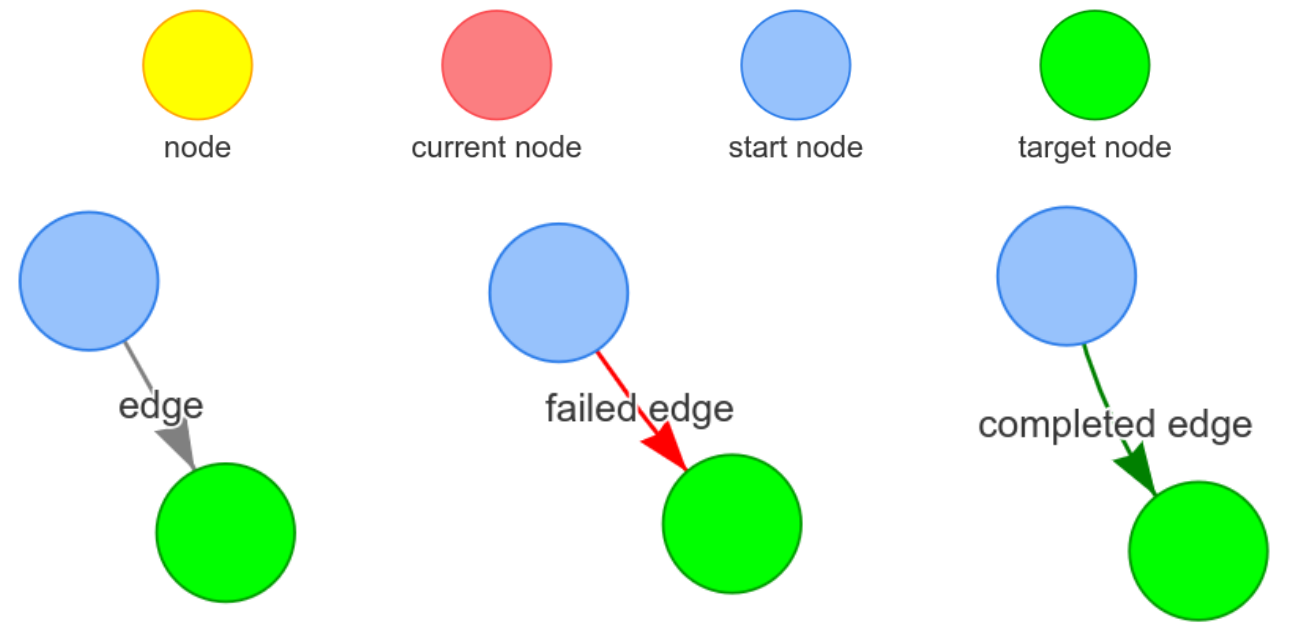
\includegraphics[width=9.6cm]{figures/proposed_method/hgraph_legend}
\end{center}
\end{frame}

% Nodes:\\
% $\gls{nodesH} = \{v_1,v_2, \dots, v_n\}$
% \vspace{0.5cm}

% Edges:\\
% $\gls{edgesH} = \{e_1,e_2, \dots, e_m\}$\bs

% $m,n \geq 0$
% \begin{textblock}{3}(1.5,1.0)
% $v_\mathit{id} =\left\langle \gls{obj}, \gls{c}(k)\right\rangle $
% \end{textblock}
% % \todo{you could make an arrow from a node to the definition of a node}

\begin{frame}[fragile]{Proposed Method: H-Graph} 
A \textbf{identification edge}: Creates a system model\bs
% \begin{equation*}
% \begin{split}
% \gls{edge}^\mathit{iden}_\mathit{id}  = & \quad \langle \mathit{id_{from}}, \mathit{id_{to}}, \textrm{ Identification method}, \textrm{ IO data set}, \\
%  & \quad \textrm{ controller}, \textrm{ system model}, \textrm{ status} \rangle
% \end{split}
% \end{equation*}

A \textbf{action edge}: \[\gls{edge}^\mathit{action}_\mathit{id} = \left\langle id_{from}, id_{to}, \textrm{ controller},\textrm{ system model}, \textrm{ path} \right\rangle\]\bs
A \textbf{empty edge}: Connect nodes that contain different objects\bs
% \[\gls{edge}^\mathit{emtpy}_\mathit{id} = \left\langle id_{from}, id_{to}, \textrm{status} \right\rangle\]\bs
\end{frame}

% \begin{frame}[fragile]{Proposed Method: H-Graph} 
% \begin{center}
% \begin{figure}[H]
% \begin{tikzpicture}[scale=0.65, every node/.style={scale=0.65}, node distance = 2cm, auto, initial]
% \centering
%     \node [state, fill=my_purple] (init) {IN};
%     \node [state, fill=my_dark_blue, below of=init] (path_exist) {PE};
%     \node [state, fill=my_light_blue, below of=path_exist] (system_model) {SM};
%     \node [state, fill=my_green, below of=system_model] (path_planned) {PP};
%     \node [state, fill=my_yellow, below of=path_planned] (executing) {EX};
%     \node [state, accepting, fill=my_orange, below of=executing] (completed) {CO};
%     \node [state, accepting, fill=my_red] (failed) at ([xshift=4cm]$(system_model)!0.5!(path_planned)$) {FAIL};

%  % arrows
%     \draw [-stealth] ([xshift=-2cm]init.west) to node[near start,above]{Select controller} (init.west);
%     \draw[-stealth] (init) edge node[left]{Path estimation} (path_exist)
%       (path_exist) edge[bend right] node[left]{Load in system model} (system_model)
% (system_model) edge[bend right] node[left]{Path planning} (path_planned)
% (path_planned) edge[bend right] node[left]{Go to execution loop} (executing)
% (executing) edge[bend right] node[left]{Completed} (completed);

%     \draw [-stealth] (init.east) [out=0, in=90] to node[xshift=0.1cm, right]{Path non-existence proven}  ([yshift=-0.03cm,xshift=0.2cm]failed.north);
%     \draw [-stealth] (path_exist.east) [out=0, in=90] to node[xshift=-0.6cm,yshift=0.55cm, above]{\shortstack[l]{System\\identification\\error}}  ([yshift=-0.03cm,xshift=-0.2cm]failed.north);
%     \draw [-stealth] (system_model.east) [out=0, in=180] to node[xshift=0.1cm, yshift=0.3cm, above]{\shortstack[l]{Path\\planning\\error}} (failed.west);
%     node[right]{path planning error}
%     ([yshift=-0.3cm]failed.west);
%     \draw [-stealth] (executing.east) [out=0, in=-90] to node[xshift=0.1cm,right]{Fault detected}(failed.south);
% \end{tikzpicture}
% \end{figure}
% \end{center}
% \end{frame}
